\subsection{Listák, felsorolások}

%49
\begin{frame}
  Háromféle felsorolás (lista) létezik a HTML-ben:
  \begin{enumerate}
    \item Számozatlan
    \item Számozott
    \item Definíciós
  \end{enumerate}
  \vfill
  Rendkívül rugalmasan formázható CSS-ből, pl. \hiv{\href{https://www.christianpinder.com/articles/menu-using-html-lists-and-css/}{weboldalak menürendszere}} is kialakítható
\end{frame}

%50
\begin{frame}
  \begin{itemize}
    \item Számozatlan felsorolás: \texttt{<ul>} (unordered list) elemmel
    \item Ennek elemei: beágyazott \texttt{<li>} (list item) elemekkel
  \end{itemize}
  \begin{columns}[T]
    \column{0.6\textwidth}
      \begin{exampleblock}{\textattachfile{bevasarlas.html}{bevasarlas.html}}
        \footnotesize
        \lstinputlisting[style=HTML,linerange={8-13},numbers=left,firstnumber=8]{bevasarlas.html}
      \end{exampleblock}
    \column{0.35\textwidth}
      \centering 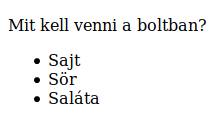
\includegraphics[width=\textwidth]{bevasarlas.png}
  \end{columns}
\end{frame}

%51
\begin{frame}
  \begin{columns}[c]
    \column{0.5\textwidth}
      Feladat: készítsen a mellékelt ábrának megfelelően egy számozatlan felsorolást tartalmazó weblapot! (Forrás: \hiv{\href{https://www.buvosszakacs.com/2014/04/13/diy-sor-bevalt-receptek/}{Bűvös Szakács}})
    \column{0.5\textwidth}
      \begin{exampleblock}{\textattachfile{sor.html}{sor.html}}
        \centering 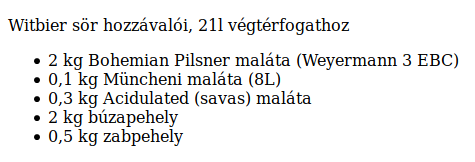
\includegraphics[width=\textwidth]{sor.png}
      \end{exampleblock}
  \end{columns}
\end{frame}

%52
\begin{frame}
  \begin{itemize}
    \item Számozott felsorolás: \texttt{<ol>} (ordered list) elemmel, attribútumai:
    \begin{description}[m]
      \item[\texttt{type}] felsorolásjel típusa \hfill \\ 
        \begin{table}[]
        \begin{tabular}{ll}
        \textbf{Att. érték} & \textbf{Felsorolásjel}       \\\hline
        1                   & Arab számok (alapértelmezés) \\
        A                   & Latin nagybetűk              \\
        a                   & Latin kisbetűk               \\
        I                   & Nagybetűs római számok       \\
        i                   & Kisbetűs római számok       
        \end{tabular}
        \end{table}
      \item[\texttt{start}] \hfill \\ Az első elem sorszáma
      \item[\texttt{reversed}] \hfill \\ Csökkenő sorrendet ír elő
    \end{description}
    \item Ennek elemei: beágyazott \texttt{<li>} (list item) elemekkel
  \end{itemize}
\end{frame}

%53
\begin{frame}
  \begin{columns}[c]
    \column{0.5\textwidth}
      \begin{exampleblock}{\textattachfile{futurama.html}{futurama.html} (\kiemelN{\href{https://www.reddit.com/r/futurama/comments/4ds4vf/what_is_this_in_reference_to/}{Futurama}})}
        \lstinputlisting[style=HTML,linerange={8-12},numbers=left,firstnumber=8]{futurama.html}
      \end{exampleblock}
    \column{0.45\textwidth}
      \begin{center}
        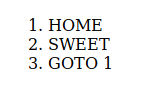
\includegraphics[width=.8\textwidth]{futurama.png}
        \vfill
        
\includegraphics[width=.8\textwidth]{futurama_orig.png}
      \end{center}
  \end{columns}
\end{frame}

%54
\begin{frame}
  \begin{columns}[c]
    \column{0.5\textwidth}
      Kiindulva a \textattachfile{jaegermeister.txt}{jaegermeister.txt} fájlból, hozza létre az ábrán látható HTML fájlt!
    \column{0.45\textwidth}
      \begin{exampleblock}{\textattachfile{jaegermeister.html}{jaegermeister.html}}
        \centering 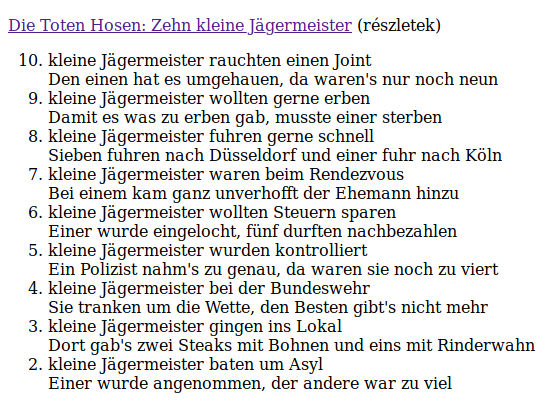
\includegraphics[width=\textwidth]{jaegermeister.png}
      \end{exampleblock}
  \end{columns}
\end{frame}

%55
\begin{frame}
  \begin{columns}[T]
    \column{0.45\textwidth}
      Többszintű felsorolások
      \begin{itemize}
        \item \texttt{<li>} elem belsejébe újabb felsorolás ágyazható
        \item A számozás újrakezdődik az első szinten $\to$ \hiv{\href{https://stackoverflow.com/questions/10405945/html-ordered-list-1-1-1-2-nested-counters-and-scope-not-working}{CSS}}
      \end{itemize}
      \vfill
      \centering 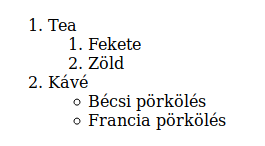
\includegraphics[width=\textwidth]{tobbszintu.png}
    \column{0.5\textwidth}
      \begin{exampleblock}{\textattachfile{tobbszintu.html}{tobbszintu.html}}
        \scriptsize
        \lstinputlisting[style=HTML,linerange={8-21},numbers=right,firstnumber=8]{tobbszintu.html}
      \end{exampleblock}
  \end{columns}
\end{frame}

%56
\begin{frame}
  \begin{itemize}
    \item Definíciós lista létrehozása \texttt{<dl>} (description list) elemmel
    \item A kifejezés megadása \texttt{<dl>}-be ágyazott \texttt{<dt>} (term) elemmel
    \item Magyarázat az ezt követő \texttt{<dd>} (description) elemben
  \end{itemize}
  \begin{columns}[T]
    \column{0.6\textwidth}
      \begin{exampleblock}{\textattachfile{froccs.html}{froccs.html}}
        \scriptsize
        \lstinputlisting[style=HTML,linerange={8-15},numbers=left,firstnumber=8]{froccs.html}
      \end{exampleblock}
    \column{0.35\textwidth}
      \centering 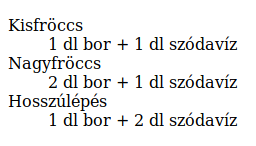
\includegraphics[width=\textwidth]{froccs.png}
  \end{columns}
\end{frame}

%57
\begin{frame}
   Hozza létre az ábrán látható HTML fájlt!
  \begin{exampleblock}{\textattachfile{betuszavak.html}{betuszavak.html}}
    \centering 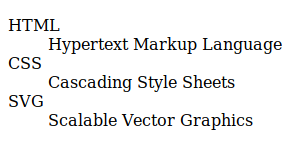
\includegraphics[scale=0.5]{betuszavak.png}
  \end{exampleblock}
\end{frame}
